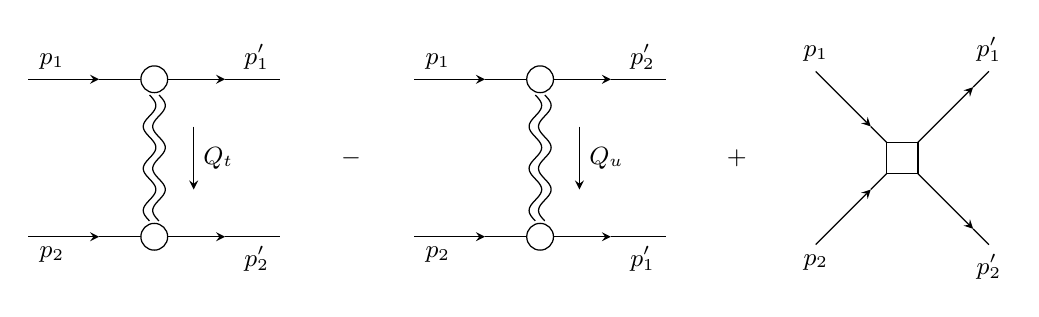
\begin{tikzpicture}[x=1mm,y=1mm,>=stealth,line width=.45pt,font=\small]
\foreach \offset/\topout/\bottomout/\mom in {0/{p'_1}/{p'_2}/{Q_t},49/{p'_2}/{p'_1}/{Q_u}} {
 \begin{scope}[shift={(\offset,0)}]
 \draw[->] (0,10)--(9,10); \draw (9,10)--(16,10);
 \draw[->] (16,10)--(25,10);\draw (25,10)--(32,10);
 \draw[->] (0,-10)--(9,-10);\draw (9,-10)--(16,-10);
 \draw[->] (16,-10)--(25,-10);\draw (25,-10)--(32,-10);
 \foreach \dx in {-0.6,0.6} {
  \draw[domain=0:1,samples=75,variable=\u]
   plot ({16+\dx+0.8*sin(\u*1080)},{8-16*\u});
 }
 \draw[->] (21,4)--(21,-4);\node[right] at(21,0){$\mom$};
 \draw[fill=white] (16,10) circle(1.7);\draw[fill=white] (16,-10) circle(1.7);
 \node[above] at(3,10){$p_1$};\node[below] at(3,-10){$p_2$};
 \node[above] at(29,10){$\topout$};\node[below] at(29,-10){$\bottomout$};
 \end{scope}
}
\node at(41,0){$-$};\node at(90,0){$+$};
\begin{scope}[shift={(100,0)}]
 \draw[->] (0,11)--(7,4);\draw (7,4)--(10,1);
 \draw[->] (0,-11)--(7,-4);\draw (7,-4)--(10,-1);
 \draw[->] (12,1)--(20,9);\draw (20,9)--(22,11);
 \draw[->] (12,-1)--(20,-9);\draw (20,-9)--(22,-11);
 \draw[fill=white] (9,-2) rectangle(13,2);
 \node[above] at(0,11){$p_1$};\node[below] at(0,-11){$p_2$};
 \node[above] at(22,11){$p'_1$};\node[below] at(22,-11){$p'_2$};
\end{scope}
\end{tikzpicture}
